\subsection{Introducción}

Go.JS \cite{gojs} es una biblioteca de JavaScript para implementar editores gráficos dentro de interfaces web. GoJS facilita la implementación de funciones tales como definición de símbolos gráficos, gestión de paletas de símbolos, arrastrar y soltar (\emph{drag and drop}), copiar y pegar, edición de etiquetas de texto asociadas a símbolos gráficos, menús contextuales, función de deshacer o gestión de eventos, entre muchas otras funcionalidades.

Para ilustrar el funcionamiento de GoJS, a continuación, se muestra un ejemplo sencillo de creación de editor gráfico de grafos para el dibujo de círculos interconectados por flechas. Dicho editor se muestra en la Figura~\ref{fig:gojssample}.

\begin{figure}[!tb]
	\centering
	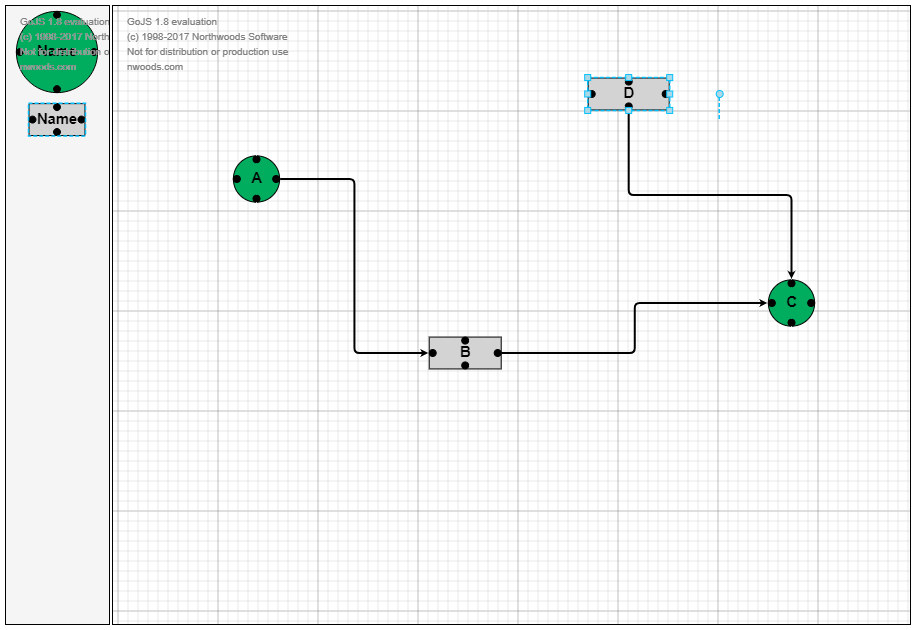
\includegraphics[scale=0.5]{gojssample.png}
	\caption{Editor gráfico creado en GoJS}
    \label{fig:gojssample}
\end{figure}

Para comenzar explicando el ejemplo, cabe destacar que, es necesario reservar dos secciones de la página HTML que lo contiene. Una sección para la paleta contenedora de los elementos gráficos del editor, que en este caso es sólo el círculo, y otra sección para el diagrama sobre el que se depositarán los elementos gráficos. 


\begin{figure}[!tb]
	\centering
	\begin{lstlisting}[language=JavaScript]
	myDiagram =
		$(go.Diagram, "myDiagramDiv",  
		{
			grid: $(go.Panel, "Grid",
				$(go.Shape, "LineH", { stroke: "lightgray", strokeWidth: 0.5 }),
				$(go.Shape, "LineH", { stroke: "gray", strokeWidth: 0.5, interval: 10 }),
				$(go.Shape, "LineV", { stroke: "lightgray", strokeWidth: 0.5 }),
				$(go.Shape, "LineV", { stroke: "gray", strokeWidth: 0.5, interval: 10 })
			),
			allowDrop: true,         
		}
	);
	\end{lstlisting}
	\caption{Creación de un Diagrama}
	\label{fig:creacionDiagrama}
\end{figure}



A continuación, se debe realizar una serie de acciones a nivel de Javascript para proporcionar tanto a la paleta de dibujo, como al área de dibujo del comportamiento deseado. En primer lugar, crearemos una variable \texttt{\$} que dé acceso al entorno GoJS. Esto se realiza mediante la llamada a la sentencia \texttt{make} de librería \emph{GraphObject} de GoJS (Figura~\ref{fig:asignacionDollar},~Línea 1).

\begin{figure}[!tb]
	\centering
	\begin{lstlisting}[language=JavaScript]
	var $ = go.GraphObject.make;
	\end{lstlisting}
	\caption{Asignación de la variable \texttt{\$}}
	\label{fig:asignacionDollar}
\end{figure}

Seguidamente, se personaliza la sección HTML reservada al diagrama, denominada \texttt{myDiagramDiv} (Figura~\ref{fig:creacionDiagrama},~Líneas~01-13), asignándole un \emph{grid} o cuadrícula de fondo (Figura~\ref{fig:creacionDiagrama},~Líneas~04-09), especificando los colores de las líneas de la cuadrícula(mediante la propiedad \emph{stroke})  y dándole la capacidad de poder arrastrar elementos sobre él (Figura~\ref{fig:creacionDiagrama},~Línea 10).

%%========================================================================%%
%% NOTE(Pablo): Hasta aquí va más o menos bien la cosa, pero aquí         %%
%%    empezamos a perder el hilo. ¿De dónde han salido los círculos y     %%
%%    qué es un puerto. Lo normal es explicar primero cómo se añaden      %%
%%    círculos a la paleta, qué es un puerto, la necesidad de crearlos,   %%
%%    y luego ya cómo se crean.                                            %% 
%%========================================================================%%
\begin{figure}[!tb]
	\centering
	\begin{lstlisting}[language=JavaScript]
	myDiagram.nodeTemplate =
		$(go.Node, "Spot",
		{ locationSpot: go.Spot.Center },
		new go.Binding("location").makeTwoWay(go.Point.stringify),
		{ selectable: true, selectionAdornmentTemplate: nodeSelectionAdornmentTemplate },
		{ resizable: true, resizeObjectName: "PANEL", resizeAdornmentTemplate: nodeResizeAdornmentTemplate },
		{ rotatable: true, rotateAdornmentTemplate: nodeRotateAdornmentTemplate },
	
		$(go.Panel, "Auto",
		{ name: "PANEL" },
		$(go.Shape,  
		{
			portId: "", 
			fromLinkable: true, toLinkable: true, cursor: "pointer",
		},
			new go.Binding("figure"),
			new go.Binding("fill")),
		$(go.TextBlock,
		{
			maxSize: new go.Size(50, 50),
			editable: true
		},
		new go.Binding("text").makeTwoWay())
		)
	);
	\end{lstlisting}
\caption{Declaración del patrón del Nodo}
\label{fig:patronNodo}
\end{figure}

La Figura~\ref{fig:patronNodo} muestra cómo se crea el patrón, o comúnmente conocido \emph{template\footnote{El template declara el conjunto de características y/o directrices que acompañan a un nodo en su creación, por ejemplo se puede definir un color concreto, o unas características que pueden ser modificadas.}}, que servirán de esqueleto para los \emph{nodos} de un diagrama. Los nodos son todos aquellos elementos de los que se va a componer el diagrama. En nuestro ejemplo, estos nodos serán círculos y rectángulos. Para crear la definición un nodo lo primero es declarar el nodo con \texttt{\$(go.Node} (Figura~\ref{fig:patronNodo},~Línea 2). 

A continuación, especificamos, mediante la definición de ciertas propiedades, cómo se comportará el nodo (Figura~\ref{fig:patronNodo},~Líneas~05-24). En nuestro caso, se indica que, dentro de las caracteristicas del nodo, podrá ser seleccionado, redimensionado y rotado (Figura~\ref{fig:patronNodo},~Líneas~05-07), además, se ha establecido una localización o situación de los puntos por defecto centrada (Figura~\ref{fig:patronNodo},~Línea~03). Junto a ella, aparece una sentencia  \emph{binding} (Figura~\ref{fig:patronNodo},~Línea~04), esta sentencia sirve para permitir en un futuro modificar dicha propiedad.

Al crear un nodo, se reserva un espacio sobre el que se van a situar los diferentes elementos del nodo, basándonos en el ejemplo, este nodo contiene un \emph{panel}(Figura~\ref{fig:patronNodo}, Línea~09), que actúa como contenedor de la figura o \emph{shape}(Figura~\ref{fig:patronNodo},~Línea~11), que es la encargada de definir la forma y otras características del nodo, como es el puerto del nodo (que actúa como identificador)(Figura~\ref{fig:patronNodo},~Línea~13) y las propiedades de enlace de las que se hablarán más adelante (Figura~\ref{fig:patronNodo},~Línea~14).

Cada nodo poseerá además una etiqueta de texto que permitirá especificar su nombre, denominada \emph{panel} (Figura~\ref{fig:patronNodo},~Línea~09). En nuestro caso, dicho panel tendrá la capacidad de poseer diferentes formas (como serán el circulo y el rectángulo) y colores gracias a los \emph{bindings} (Figura~\ref{fig:patronNodo},~Líneas~16-17). 

Una vez definidas las propiedades básicas de un nodo, el siguiente paso es definir cómo enlazar dichos nodos. Para ello debemos definir dos elementos: \emph{puertos} y \emph{enlaces}. Los puertos de un nodo son los puntos de un nodo desde los cuáles dicho nodo se puede enlazar con otros nodos. Para añadir puertos a los círculos creamos una función determinada, la cual se muestra en la Figura \ref{}. %% Describir algo del código que aparece. 
A continuación, añadimos cuatro llamadas a esta función a la declaración de los círculos como nodos, con el objeto de crear un puerto a cada lado del eje de un círculo (Figura~\ref{}).

%%=========================================================================%%
%% NOTE(Pablo): La figura donde se añaden los cuatro makePort hay que      %%
%%   hacerla nueva                                                         %%
%%=========================================================================%%

%%=========================================================================%%
%% NOTE(Pablo): ¿Por qué los parámetros tres y cuatro cambiando de true    %%
%%   a false a veces?                                                      %%
%%=========================================================================%%

\begin{figure}[!tb]
	\centering
	\begin{lstlisting}[language=JavaScript]
	myDiagram.linkTemplate =
		$(go.Link, 
			$(go.Shape,  
			{ isPanelMain: true, strokeWidth: 2 }),
			$(go.Shape,  
			{ toArrow: "Standard", stroke: null }
		)
	)
	\end{lstlisting}
\caption{Declaración del patrón del Link}
\label{fig:patronlink}
\end{figure}

Una vez definidos los puertos, especificamos cómo se comportarán los enlaces entre nodos, tal como muestra la Figura~\ref{}. %% Comentar un poco más aquí sobre el código.


\begin{figure}[!tb]
	\centering
\begin{lstlisting}[language=JavaScript]
myPalette =
	$(go.Palette, "myPaletteDiv",  
	{
		nodeTemplateMap: myDiagram.nodeTemplateMap,  
		linkTemplate: 
		$(go.Link,
			$(go.Shape, 
			{ isPanelMain: true, strokeWidth: 2 }),
			$(go.Shape,  
			{ toArrow: "Standard", stroke: null })
		),
		model: new go.GraphLinksModel([  
			{ text: "Name", figure: "Circle", fill: "#00AD5F" },
			{ text: "Name", figure: "Rectangle", fill: "lightgray" }
			])
		}
);
\end{lstlisting}
\caption{Creación de la Paleta de Nodos}
\label{fig:paletaNodos}
\end{figure}

Por último, creamos la paleta de herramienta, tal como se muestra en la Figura~\ref{}. Como se puede observar, la paleta se sitúa sobre una sección HTML denominada \emph{myPalleteDiv}. 

%% A dicha paleta asocia  los nodos y se le añade al modelo de datos de la paleta un elemento círculo de color verde y sin texto en su interior.

Una vez definidos estos elementos, nuestro editor gráfico queda implementado ya que GoJS se encargará de dibujar los elementos sobre el área de dibujo cuando estos son seleccionados en la paleta, permitiendo arrastrarlos, redimensionarlos o renombrarlos, entre otras funciones. Por tanto, GoJS nos permite obtener fácilmente editores gráficos en Javascript a partir de la especificación
de las propiedades que compondrán dicho editor. Concretamente, el editor de la Figura~\ref{} se puede implementar con sólo XX líneas Javascript.     